\documentclass[14pt]{memoir}

\usepackage{geometry}
\usepackage[utf8]{inputenc}
\usepackage{amsmath}
\usepackage{amsfonts}
\usepackage{amssymb}
\usepackage{graphicx}
\usepackage[utf8]{inputenc}
\usepackage{amsmath}
\usepackage{amsfonts}
\usepackage{amssymb}
\usepackage[shortlabels]{enumitem}
\usepackage{listings}
\usepackage{xcolor}
\usepackage[most]{tcolorbox}
\usepackage{mathtools}
\usepackage{float}
\usepackage[colorlinks=false, linktocpage=true]{hyperref}

\usepackage{booktabs}% http://ctan.org/pkg/booktabs
\newcommand{\tabitem}{~~\llap{\textbullet}~~}
\usepackage{longtable}
 
\usepackage{caption}
\DeclareCaptionType{code}[Code Listing][List of Code Listings] 

\definecolor{codegreen}{rgb}{0,0.6,0}
\definecolor{codegray}{rgb}{0.5,0.5,0.5}
\definecolor{codepurple}{rgb}{0.58,0,0.82}
\definecolor{backcolour}{rgb}{0.95,0.95,0.92}
 
\lstdefinestyle{mystyle}{
    backgroundcolor=\color{backcolour},   
    commentstyle=\color{codegreen},
    keywordstyle=\color{magenta},
    numberstyle=\tiny\color{codegray},
    stringstyle=\color{codepurple},
    basicstyle=\ttfamily\footnotesize,
    breakatwhitespace=false,         
    breaklines=true,                 
    captionpos=b,                    
    keepspaces=true,                 
    numbers=left,                    
    numbersep=5pt,                  
    showspaces=false,                
    showstringspaces=false,
    showtabs=false,                  
    tabsize=2
}
 
\lstset{style=mystyle}

\setlength{\parindent}{0em}
\setlength{\parskip}{1em}

\author{Brian Rashap, Ph.D.}
\title{ENGR2910 - Circuit Analysis I}

\geometry{letterpaper, portrait, margin=0.75in}

\begin{document}
\frontmatter

\maketitle


\mainmatter

\chapter{Circuit Variables}

\section{Electrical Engineering: An Overview}

\begin{figure}[h]
\begin{center}
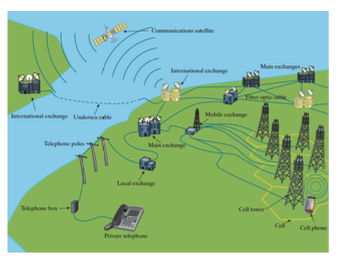
\includegraphics[scale=0.40]{fig/fig01_01.png}
\caption{Telephone System}
\label{fig:01_01}
\end{center}
\end{figure}

Five classifications of electrical systems:
\begin{enumerate}
\item Communication Systems
\item Computer Systems
\item Control Systems
\item Power Systems
\item Signal-Processing Systems
\end{enumerate}

\subsection{Circuit Theory}
Three assumptions:
\begin{itemize}
\item Electrical effects happen instantaneously throughout a system; tis assumption is called the lumped-parameter system)
\item The net charge on every component in the system is always zero.
\item There is not magnetic coupling between the components of a system. However, we will allow magnetic coupling within a component.
\end{itemize}

\section{International System of Units}

\begin{figure}[h]
\begin{center}
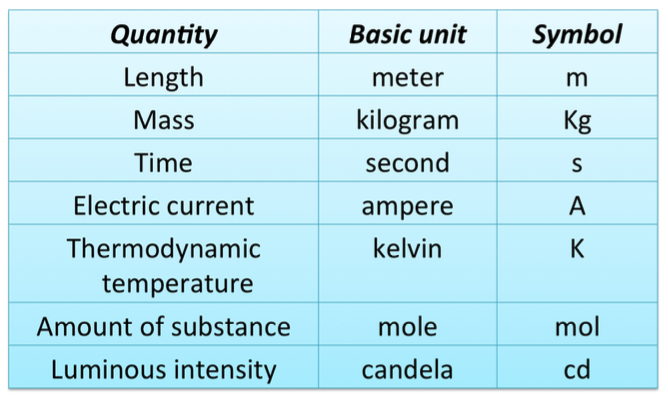
\includegraphics[scale=0.30]{fig/tab01_01.png}
\caption{Scientific Units}
\label{fig:t01_01}
\end{center}
\end{figure}

\begin{figure}[h]
\begin{center}
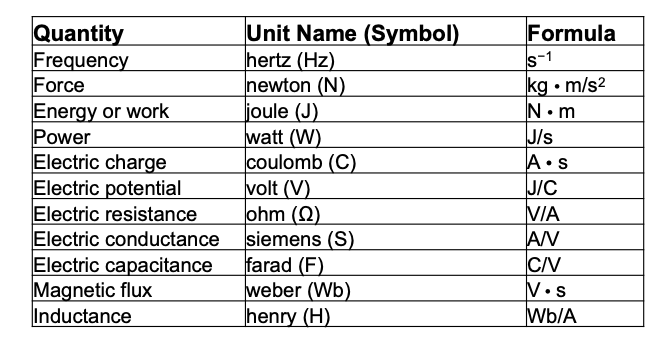
\includegraphics[scale=0.40]{fig/tab01_02.png}
\caption{Derived Units}
\label{fig:t01_02}
\end{center}
\end{figure}

\begin{figure}[!h]
\begin{center}
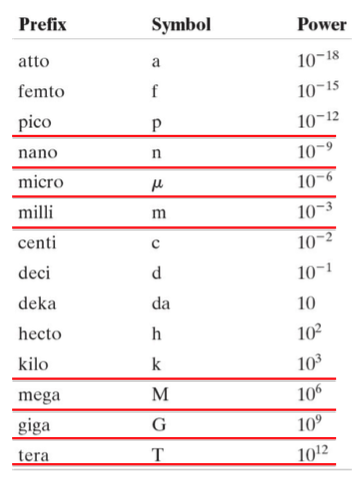
\includegraphics[scale=0.40]{fig/tab01_03.png}
\caption{Powers of 10}
\label{fig:t01_03}
\end{center}
\end{figure}

\subsection{Circuit Analysis: An Overview}

All engineering designs begin with a need that may include a Circuit Model before a physical prototype:

\begin{figure}[h]
\begin{center}
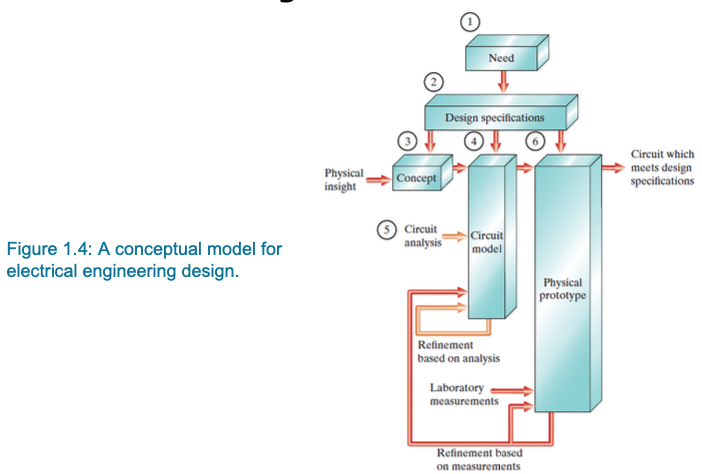
\includegraphics[scale=0.65]{fig/fig01_04.png}
\caption{Conceptual Model for Electrical Engineering Design}
\label{fig:f01_04}
\end{center}
\end{figure}

\subsection{Voltage and Current}

Definition of Voltage ($v$)
\begin{equation}
v = \frac{dw}{dq}
\end{equation}
where w is energy in joules and q is the charge in coulombs. Note that the charge of one electron ($e$ is
\begin{equation}
e = 1.60022 \times 10^{-19} C
\end{equation}

Definition of Current ($i$)
\begin{equation}
i = \frac{dq}{dt},
\end{equation}
where q is charge in coulombs and t is time in seconds.

Note, the direction of current is defined by the direction of flow of positive charge. 

\subsection{DC vs AC}

Direct current is constant with time.
Alternating current varies (sinusoidally) with time and reverses direction

\begin{figure}[h]
\begin{center}
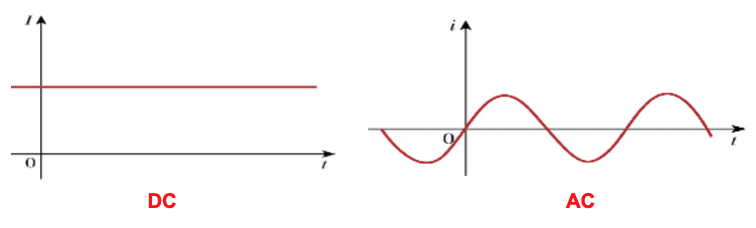
\includegraphics[scale=0.40]{fig/fig01_04a.png}
\caption{DC vs AC}
\label{fig:f01_04a}
\end{center}
\end{figure}

\subsection{Ideal Basic Circuit Element}

The ideal circuit element has three attributes:
\begin{enumerate}
\item It has only two terminals
\item It is described mathematically in terms of current and/or voltage
\item It can not be subdivided to make other elements
\end{enumerate}

\begin{figure}[h]
\begin{center}
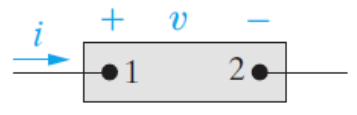
\includegraphics[scale=0.40]{fig/fig01_05.png}
\caption{Ideal basic circuit element}
\label{fig:f01_05}
\end{center}
\end{figure}


\subsubsection{WARNING: Positive Sign Convention}

Whenever the reference direction for the current in an element is in the direction of the reference voltage drop across the element, use a positive sign in any expression that relates he voltage to current. 

\section{Power and Energy}

Power is the energy per unit time

\begin{equation}
p = \frac{dw}{dt},
\end{equation}
where $p$ s power in watts, $w$ is energy in joules, and $t$ is time in seconds. And, where $1W = 1 \frac{J}{s}$.

\begin{equation}
p = \frac{dw}{dt} = (\frac{dw}{dq}) (\frac{dq}{dt})
\end{equation}

therefore,
\begin{equation}
p = v i
\end{equation}

Note, by convention, power is positive ($p>0$) if power is being delivered, and power is negative if power is being extracted from the circuit. 


\subsubsection{Law of Conservation of Energy}

\begin{equation}
\sum p = 0
\end{equation}

Energy is the capacity to do work (measured in J)

\begin{equation}
w = \int_{t_0}^t p dt = \int_{t_0}^t  v i dt
\end{equation}



\begin{figure}[h]
\begin{center}
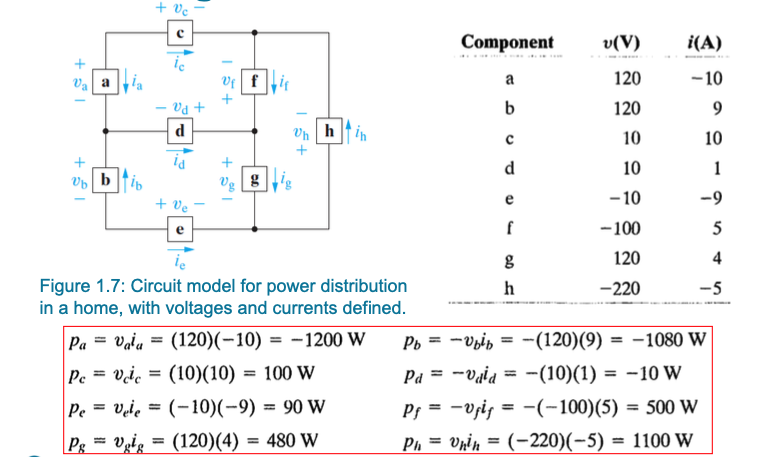
\includegraphics[scale=0.60]{fig/fig01_07a.png}
\caption{Balancing Power Example}
\label{fig:f01_07a}
\end{center}
\end{figure}


\begin{figure}[h]
\begin{center}
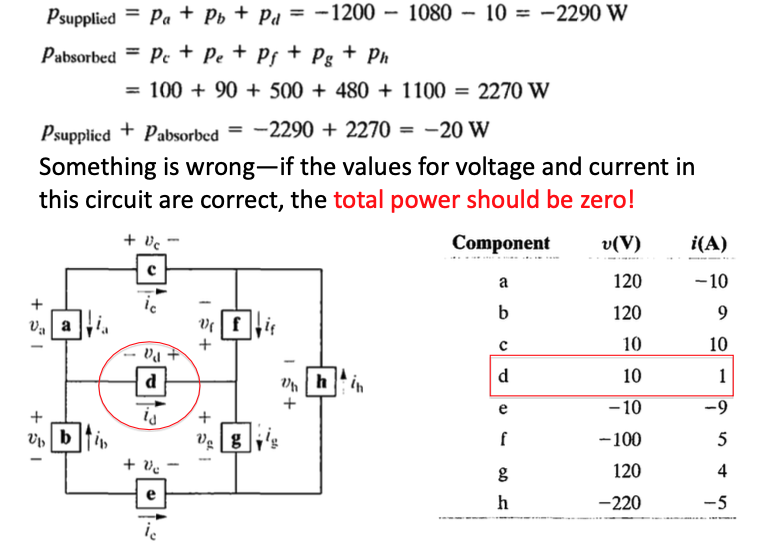
\includegraphics[scale=0.60]{fig/fig01_07b.png}
\caption{Balancing Power Correction}
\label{fig:f01_07b}
\end{center}
\end{figure}

\chapter{Circuit Elements}

\section{Voltage and Current Sources}


When we speak of circuit elements, it is important to differentiate between the physical device itself and the mathematical model which we will use to analyze its behavior in a circuit. We will use the expression circuit element to refer to the mathematical model. All the simple circuit elements that we will consider can be classified according to the relationship between current through the element to the voltage across the element.

\subsection{Ideal Sources}
\begin{itemize}
\item Ideal voltage source is a circuit element that maintains a prescribed voltage across its terminals regardless of the current flowing in those terminals. 
\item Ideal current source is a circuit element that maintains a prescribed current through its terminals regardless of the voltage across those terminals.
\end{itemize}

\begin{figure}[h]
\begin{center}
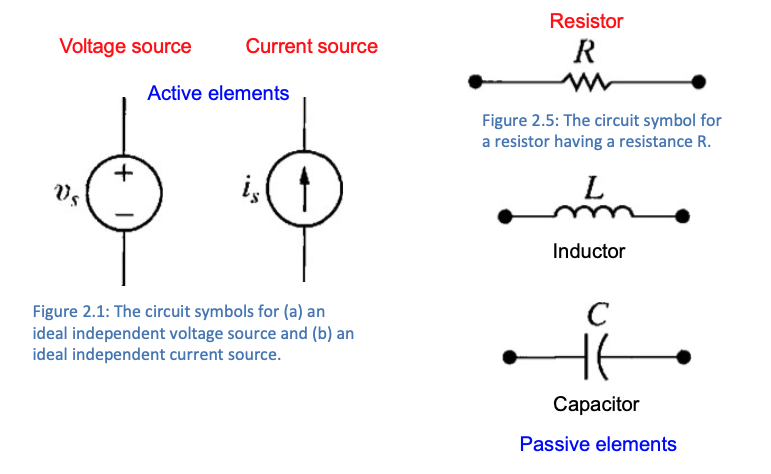
\includegraphics[scale=0.60]{fig/fig02_01.png}
\caption{Five Basic Circuit Elements}
\label{fig:f02_01}
\end{center}
\end{figure}

\subsection{Independent and Dependent Sources}

An independent source establishes a voltage or current in a circuit without relying on voltage or currents elsewhere in the circuit. 

A dependent source establishes a voltage or current whose value depends on the value of a voltage or current elsewhere in the circuit. You cannot specify the value of a dependent source unless you know the value of the voltage or current on which it depends.

There are four kinds of controlled sources:
\begin{itemize}
\item current-controlled current source (CCCS)
\item voltage-controlled current source (VCCS)
\item voltage-controlled voltage source, (VCVS)
\item current-controlled voltage source, (CCVS)
\end{itemize}

\begin{figure}[h]
\begin{center}
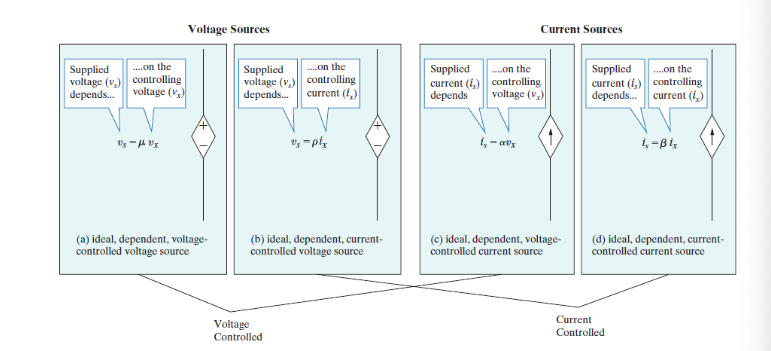
\includegraphics[scale=0.60]{fig/fig02_02.png}
\caption{Four Controlled Sources}
\label{fig:f02_02}
\end{center}
\end{figure}

\section{Electrical Resistance (Ohm's Law)}
Resistance is the capacity of materials to impede the flow of current or, more specifically, the flow of electric charge. The circuit element used to model this behavior is the resistor. The linear resistor is the simplest passive element.

\subsection{Ohm's Law}
The relationship between Voltage and Current was empirically determined by Goerg Ohm\footnote{A presented in a paper published in 1827}

\begin{figure}[H]
\begin{center}
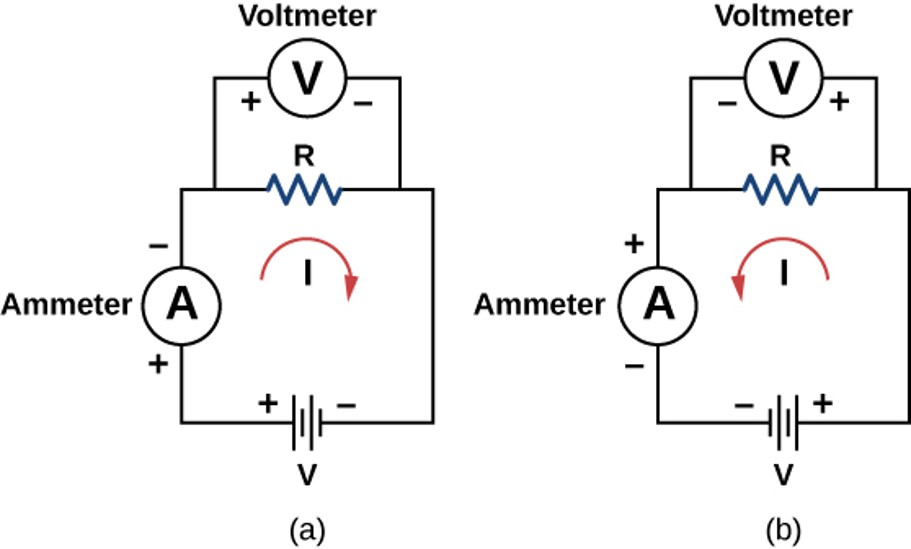
\includegraphics[scale=0.50]{fig/fig_09_19.jpg}
\caption{Goerg Ohm's Setup}
\label{fig:09_19}
\end{center}
\end{figure}

\begin{figure}[H]
\begin{center}
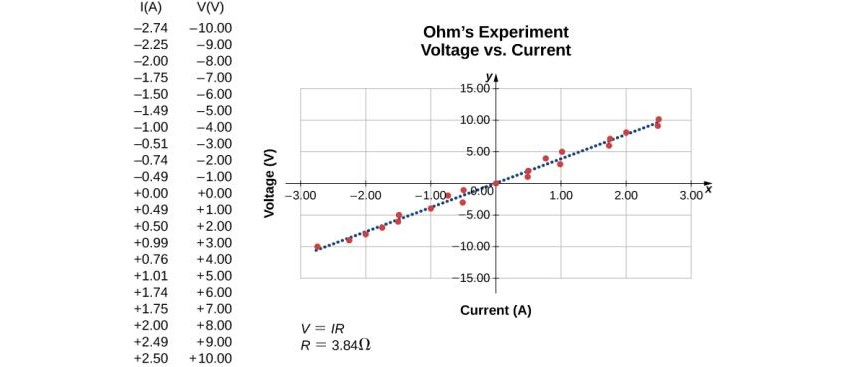
\includegraphics[scale=0.50]{fig/fig_09_20.jpg}
\caption{Goerg Ohm's Data}
\label{fig:09_20}
\end{center}
\end{figure}

Ohm's Law
\begin{equation}
v = i \cdot R
\end{equation}

\subsection{Power}

\begin{equation}
p = vi
\end{equation}

Therefore:

\begin{equation}
p = (iR) i = i^2 R
\end{equation}

or

\begin{equation}
p = v \frac{v}{R} = \frac{v^2}{R}
\end{equation}

Why is this important?

\begin{figure}[H]
\begin{center}
\includegraphics[scale=1]{fig/transistorVoltage.png}
\caption{Why Care About Voltage}
\label{fig:tv}
\end{center}
\end{figure}

\section{Constructing a circuit model}

\begin{figure}[H]
\begin{center}
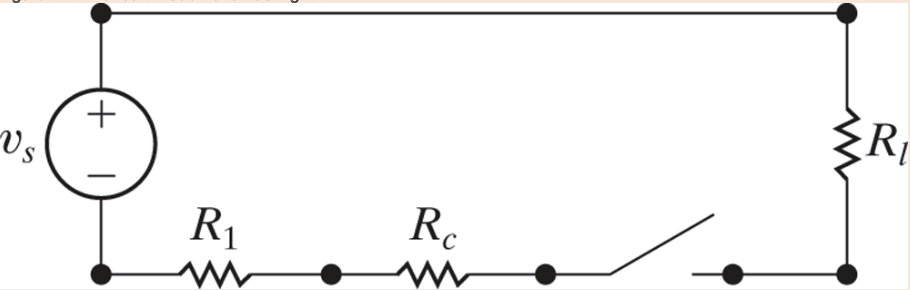
\includegraphics[scale=0.50]{fig/fig02_12.png}
\caption{Flashlight}
\label{fig:fig02_12}
\end{center}
\end{figure}

\begin{itemize}
\item Dry Cell Batteries
\item Lamp ($R_l$)
\item Switch
\item Case ($R_c$)
\item Connector Spring ($R_s$)
\end{itemize}


\section{Kirchhoff's Laws}

\subsection{Kirchhoff's First Law (the Node Law or the Junction Rule)} 
The sum of all currents entering a junction must equal the sum of all currents leaving the junction.

\begin{figure}[H]
\begin{center}
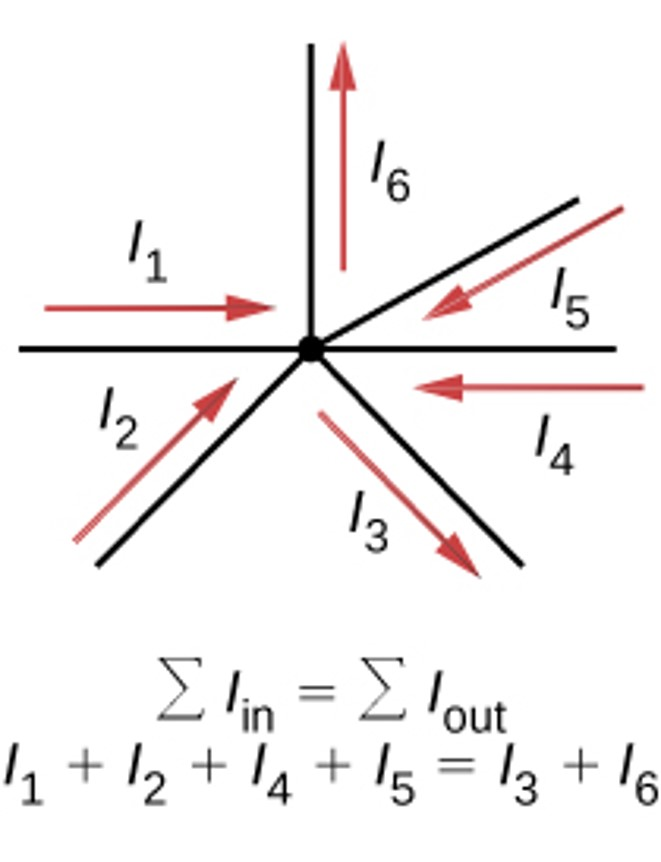
\includegraphics[scale=0.50]{fig/fig_10_20.jpg}
\caption{Kirchholff's Node Law}
\label{fig:10_20}
\end{center}
\end{figure}

\begin{equation}
\sum I_{in} = \sum I_{out}
\end{equation}

\begin{figure}[H]
\begin{center}
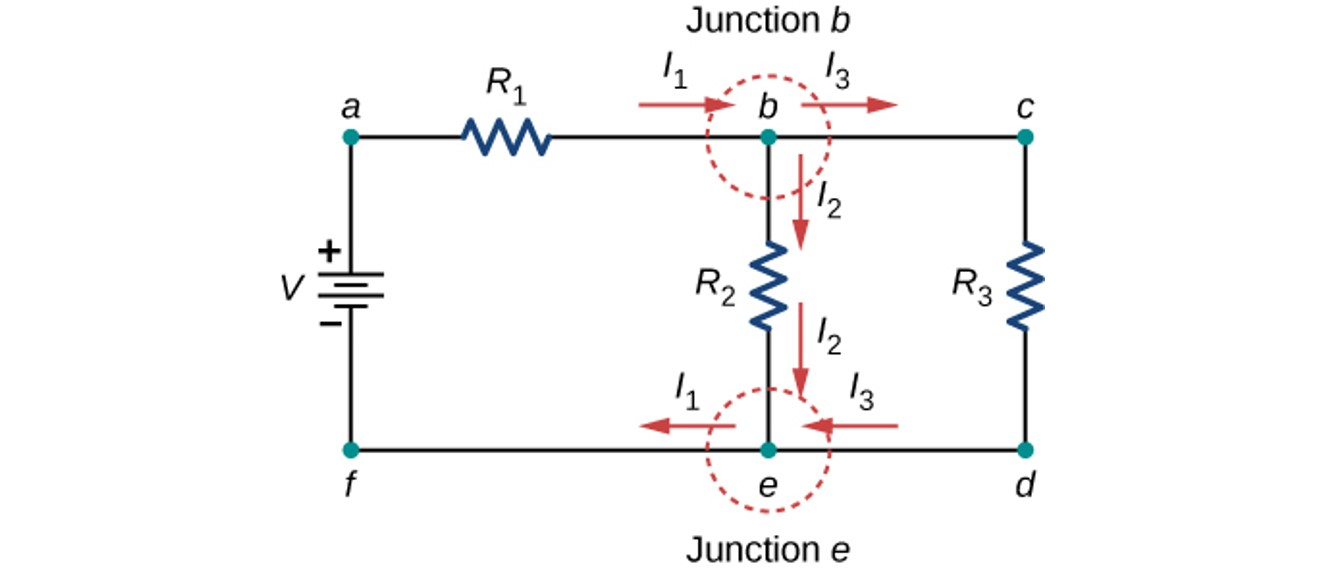
\includegraphics[scale=0.50]{fig/fig_10_24.jpg}
\caption{Kirchholff's Node Law Example}
\label{fig:10_24}
\end{center}
\end{figure}

\subsection{Kirchhoff's Second Law (the Loop Law or the Loop Rule)}

The sum off all potential differences, including those supplied by voltage sources and resistive elements, around a closed loop equals zero.

\begin{figure}[H]
\begin{center}
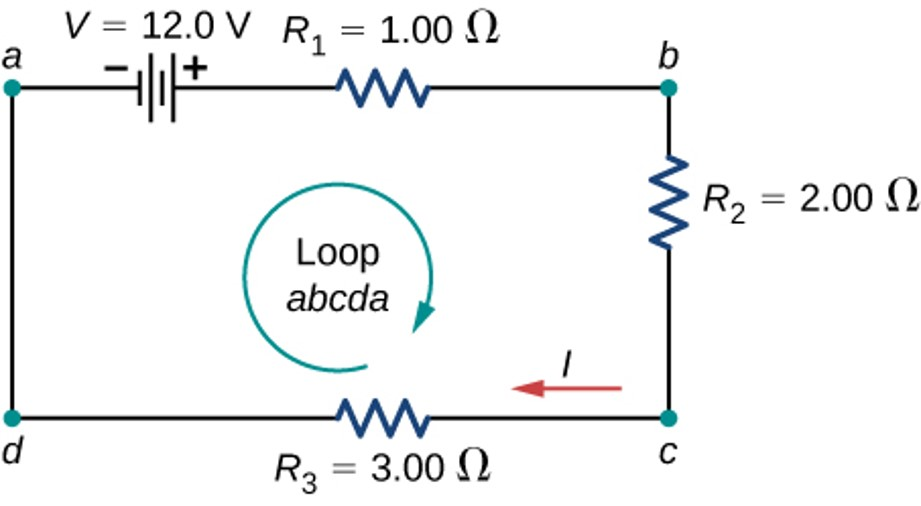
\includegraphics[scale=0.50]{fig/fig_10_21.jpg}
\caption{Kirchholff's Loop Law}
\label{fig:10_21}
\end{center}
\end{figure}

\begin{equation}
\sum_{closed loop} V = 0
\end{equation}

\begin{figure}[H]
\begin{center}
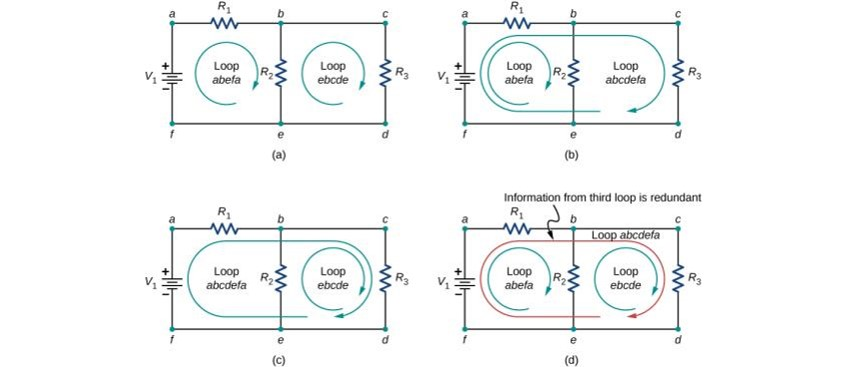
\includegraphics[scale=0.50]{fig/fig_10_25.jpg}
\caption{Kirchholff's Loop Law Example}
\label{fig:10_25}
\end{center}
\end{figure}

\section{Kirchhoff Examples}

\begin{figure}[H]
\begin{center}
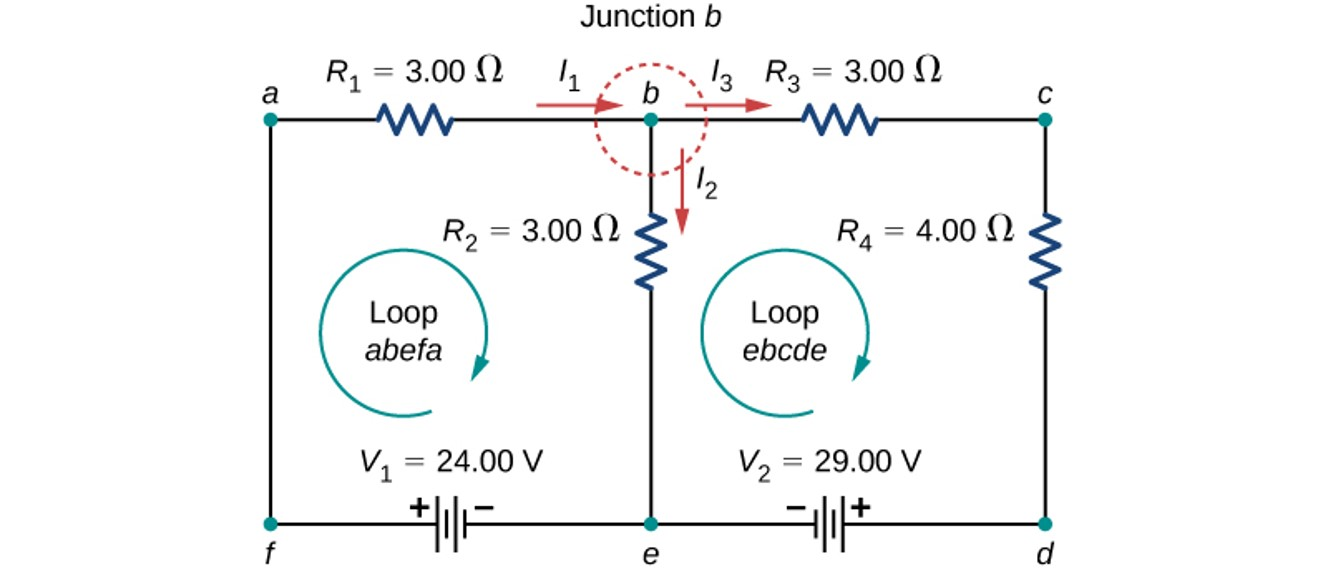
\includegraphics[scale=0.50]{fig/fig_10_28.jpg}
\caption{Kirchholff Example}
\label{fig:10_28}
\end{center}
\end{figure}

\begin{figure}[H]
\begin{center}
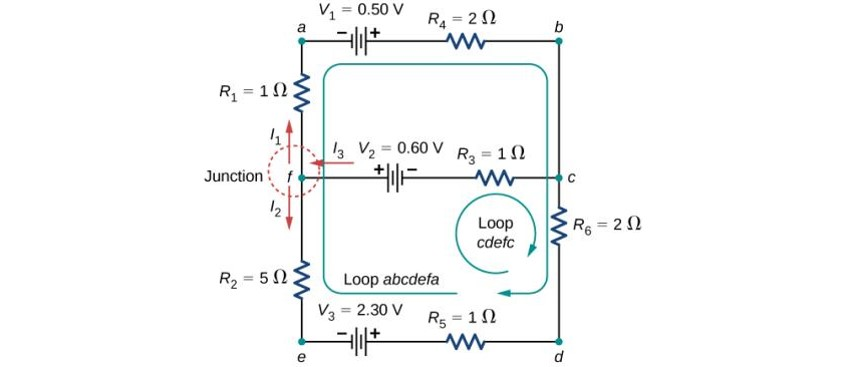
\includegraphics[scale=0.50]{fig/fig_10_29.jpg}
\caption{Kirchholff Examples}
\label{fig:10_29}
\end{center}
\end{figure}

\section{Circuits Containing Dependent Sources}

\begin{figure}[H]
\begin{center}
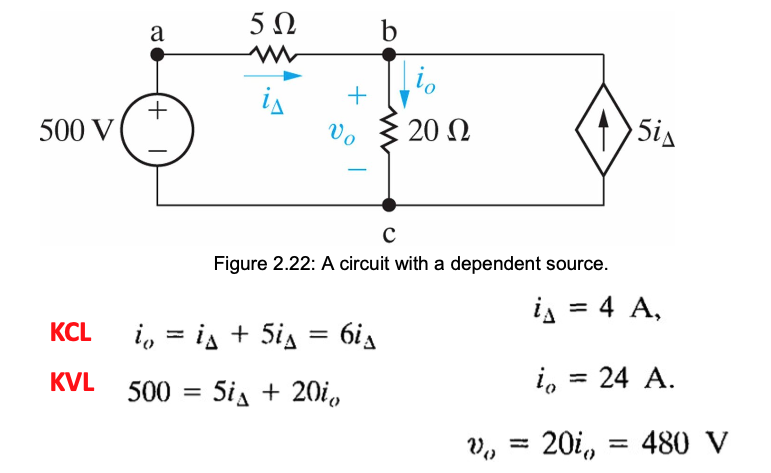
\includegraphics[scale=0.50]{fig/fig02_22.png}
\caption{Controlled Sources}
\label{fig:fig02_22}
\end{center}
\end{figure}


\chapter{Simple Resistive Circuits}

\section{Resistors in Series}

\begin{figure}[H]
\begin{center}
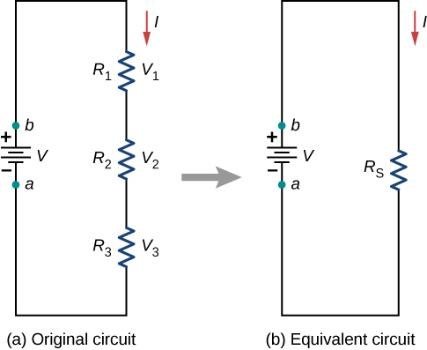
\includegraphics[scale=0.50]{fig/fig_10_12.jpg}
\caption{Resistors in Series}
\label{fig:10_12}
\end{center}
\end{figure}

For resistors in Series

\begin{equation}
V = V_1 + V_2 + V_3
\end{equation}

\begin{equation}
V = 1R_1 + 1R_2 + 1R_3
\end{equation}

\begin{equation}
I = \frac{V}{R_1 + R_2 + R_3}
\end{equation}

So

\begin{equation}
R_{eq} = \sum_{i=1}^{N} R_i
\end{equation}

\begin{figure}[H]
\begin{center}
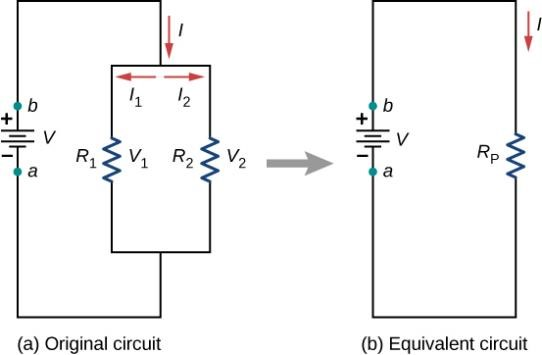
\includegraphics[scale=0.50]{fig/fig_10_14.jpg}
\caption{Resistors Parallel}
\label{fig:10_14}
\end{center}
\end{figure}

\section{Resistors in Parallel}

\begin{equation}
V = V_1 = V_2
\end{equation}

\begin{equation}
I = I_1 + I_2
\end{equation}

\begin{equation}
\frac{V}{R_{eq}} = \frac{V_1}{R_1} + \frac{V_2}{R_2}
\end{equation}

Because the Voltage is equal across the resistors
\begin{equation}
\frac{1}{R_{eq}} = \frac{1}{R_1} + \frac{1}{R_2}
\end{equation}

Or, more generically

\begin{equation}
R_{eq} = (\sum_{i=1}{N} \frac{1}{R_i})^{-1}
\end{equation}



\begin{figure}[H]
\begin{center}
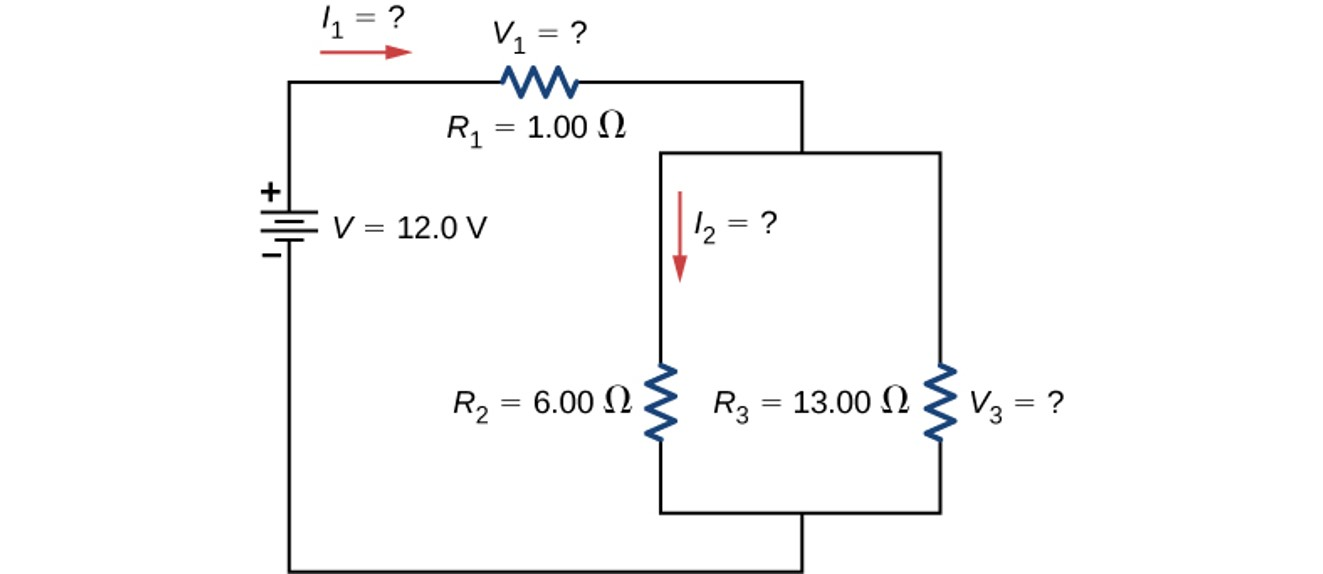
\includegraphics[scale=0.50]{fig/fig_10_16.jpg}
\caption{Resistors in Series and Parallel}
\label{fig:10_16}
\end{center}
\end{figure}

\begin{tcolorbox}
Do Example 3.1 and Example 3.2
\end{tcolorbox}



\section{Divider Circuits}

\begin{figure}[H]
\begin{center}
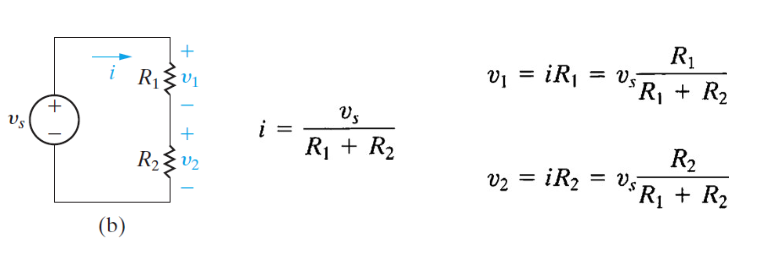
\includegraphics[scale=0.50]{fig/fig03_14.png}
\caption{Voltage Divider}
\label{fig:fig03_14}
\end{center}
\end{figure}

\begin{tcolorbox}
Do Example 3.3
\end{tcolorbox}



\begin{figure}[H]
\begin{center}
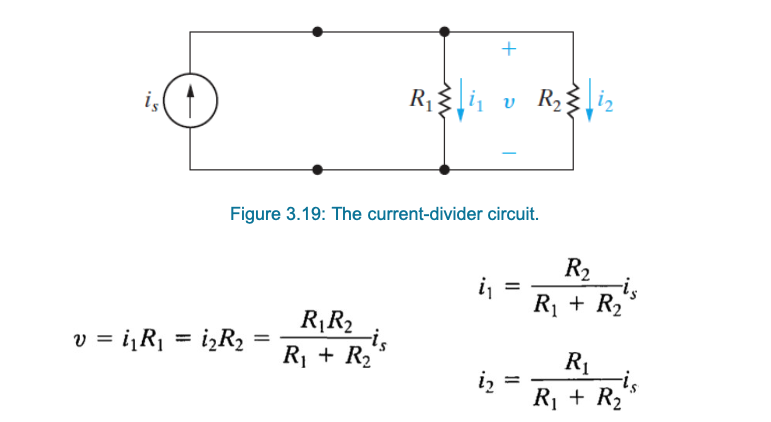
\includegraphics[scale=0.50]{fig/fig03_19.png}
\caption{Current Divider}
\label{fig:fig03_19}
\end{center}
\end{figure}

\begin{tcolorbox}
Do Example 3.6
\end{tcolorbox}


\subsection{With a Load}

\begin{figure}[H]
\begin{center}
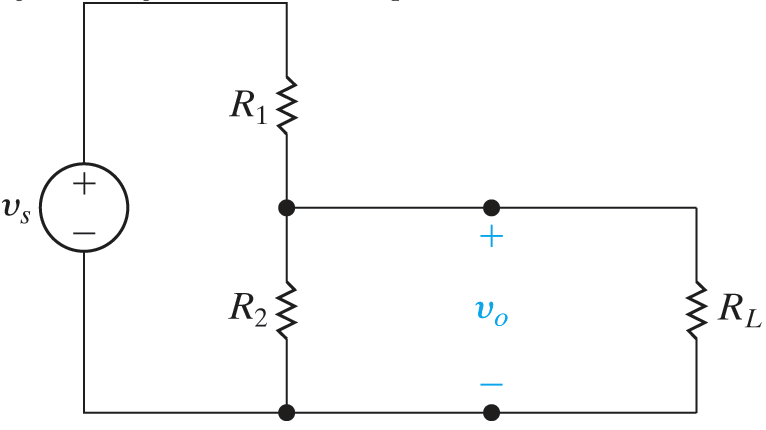
\includegraphics[scale=0.50]{fig/fig03_17.png}
\caption{Voltage Divider with Load}
\label{fig:fig03_17}
\end{center}
\end{figure}

\begin{equation}
v_0 = \frac{R_{eq}}{R_1+R_{eq}} v_s
\end{equation}

where

\begin{equation}
R_{eq} = \frac{R_2 R_L}{R_2 + R_L}
\end{equation}

substituting 

\begin{equation}
v_0 = \frac{R_2}{R_1 [1 + \frac{R_2}{R_L}] + R_2} v_s
\end{equation}

\section{Measuring Voltage and Current}

\begin{itemize}
\item An ammeter is an instrument designed to measure current; it is placed in series with the circuit element whose current is being measured. 
\item A voltmeter is an instrument designed to measure voltage; it is placed in parallel with the circuit element whose current is being measured. 
\end{itemize}

\begin{figure}[H]
\begin{center}
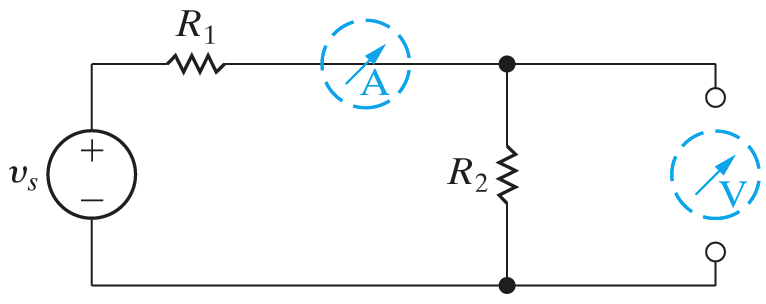
\includegraphics[scale=0.50]{fig/fig03_24.png}
\caption{Short-circuit model for ideal ammeter, and open-circuit model for ideal volt meter}
\label{fig:fig03_24}
\end{center}
\end{figure}

\subsection{d'Arsonval meter}

\begin{figure}[H]
\begin{center}
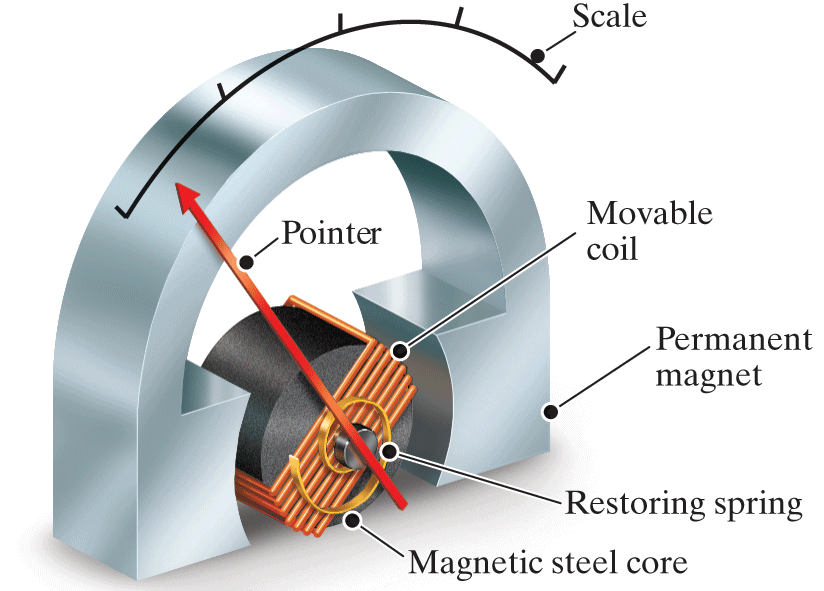
\includegraphics[scale=0.50]{fig/fig03_25.png}
\caption{d'Arsonval meter movement}
\label{fig:fig03_25}
\end{center}
\end{figure}

\subsection{Non-ideal meters}

\begin{figure}[H]
\begin{center}
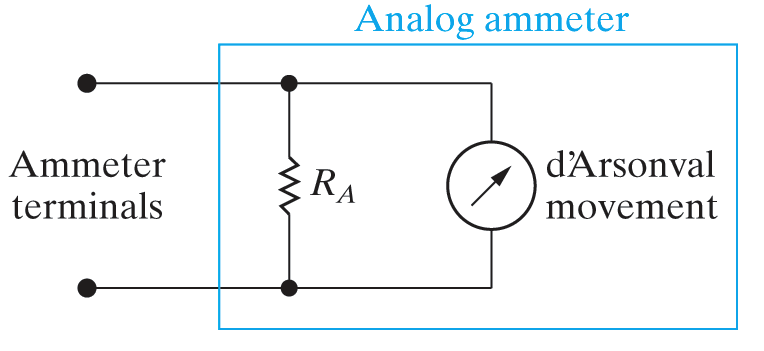
\includegraphics[scale=0.60]{fig/fig03_26.png}
\caption{Non-Ideal Ammeter}
\label{fig:fig03_26}
\end{center}
\end{figure}

\begin{figure}[H]
\begin{center}
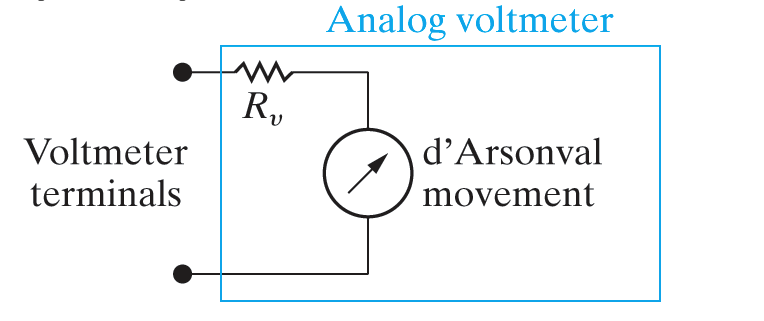
\includegraphics[scale=0.60]{fig/fig03_27.png}
\caption{Non-ideal Voltmeter}
\label{fig:fig03_27}
\end{center}
\end{figure}


\subsection{The Wheatstone Bridge}
The Wheatstone Bridge\footnote{Sir Charles Wheatstone (6 February 1802 – 19 October 1875), was an English scientist and inventor of many scientific breakthroughs of the Victorian era.  Wheatstone is best known for his contributions in the development of the Wheatstone bridge, originally invented by Samuel Hunter Christie, which is used to measure an unknown electrical resistance} is one, of many, configurations that can be used to measure resistance. 

\begin{figure}[H]
\begin{center}
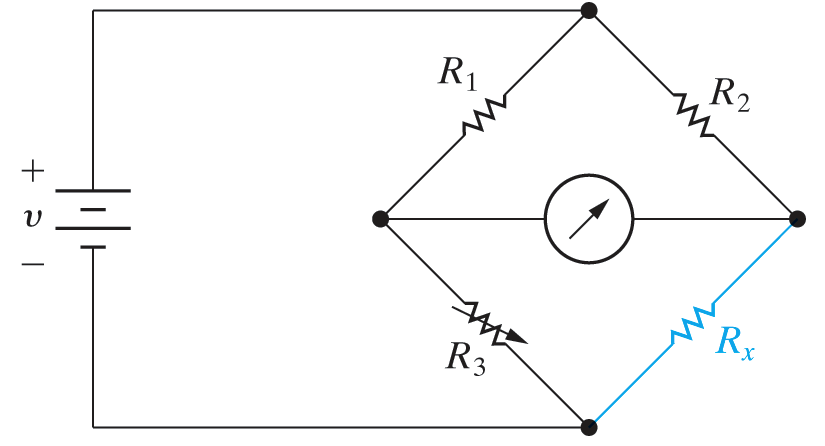
\includegraphics[scale=0.50]{fig/fig03_28.png}
\caption{Wheatstone Bridge}
\label{fig:fig03_28}
\end{center}
\end{figure}

To find $R_x$, the variable resistor $R_3$ is adjusted until t here is no current in the galvanometer.  Then the value of unknown resistor can be found by

\begin{equation}
R_x = \frac{R_2}{R_1}R_3
\end{equation}

\subsection{Derivation using Kirchhoff's Laws}

\begin{figure}[H]
\begin{center}
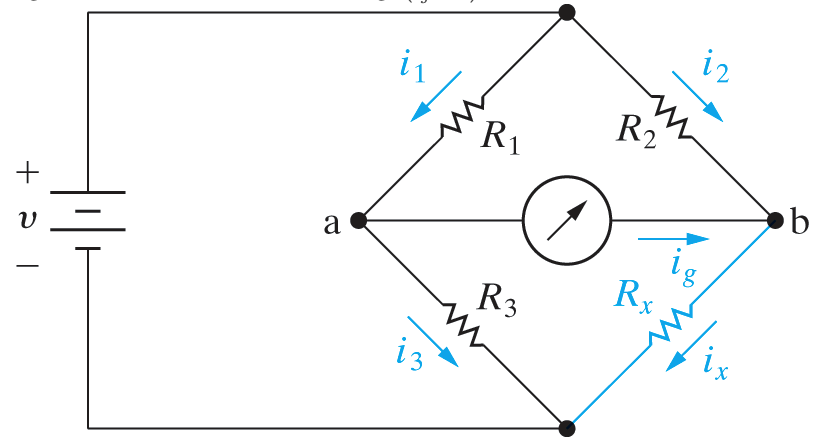
\includegraphics[scale=0.50]{fig/fig03_29.png}
\caption{Balanced Wheatstone Bridge}
\label{fig:fig03_29}
\end{center}
\end{figure}

Using KCL, since $i_g = 0$, at Node A:

\begin{equation}
i_1 = i_3
\end{equation}

And, at Node B:

\begin{equation}
i_2 = i_x
\end{equation}

Because $i_g = 0$, this also implies the voltage drop across the detector is also zero, and thus Nodes A and B are at the same potential. 

From KVL:

\begin{equation}
 i_3 R_3 - i_x R_x = 0
\end{equation}
or
\begin{equation}
i_3 R_3 = i_x R_x
\end{equation}

Likewise,
\begin{equation}
i_1 R_1 = i_2 R_2
\end{equation}

Divide the first KVL equation by the second

\begin{equation}
\frac{i_3 R_3}{i_1 R_1} = \frac{i_x R_x}{i_2 R_2}
\end{equation}

Since $i_1 = i_3$ and $i_2 = i_x$, solving for $R_x$:

\begin{equation}
R_x = \frac{R_2}{R_1}R_3
\end{equation}

\begin{tcolorbox}
Do Example 3.10
\end{tcolorbox}


\section{Delta-to-Wye (Pi-to-Tee) Equivalent Circuits}

The $\Delta$ and $Y$structures are present in a variety of useful circuits. Hence, the $\Delta-Y$  transformation is helpful in circuit analysis. 

\begin{figure}[H]
\begin{center}
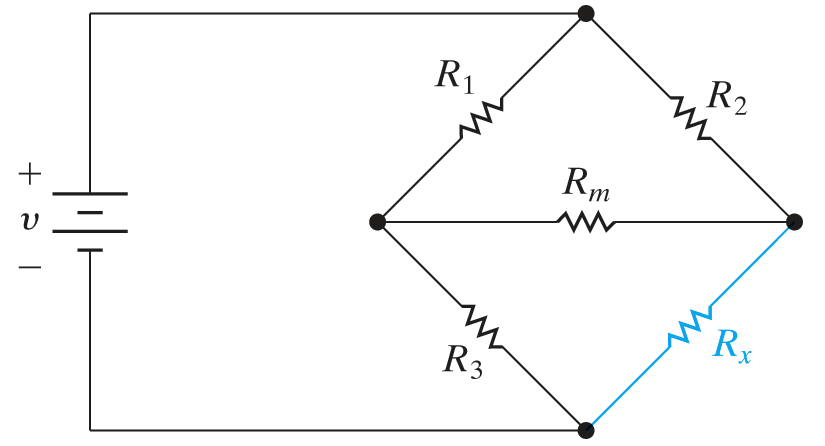
\includegraphics[scale=0.50]{fig/fig03_31.png}
\caption{Resistive Network generated by a Wheatstone Bridge circuit}
\label{fig:fig03_31}
\end{center}
\end{figure}

Resistors $R_1$, $R_2$, and $R_m$ (or $R_3$, $R_x$, and $R_m$) form a delta ($\Delta$) interconnect. 

\begin{figure}[H]
\begin{center}
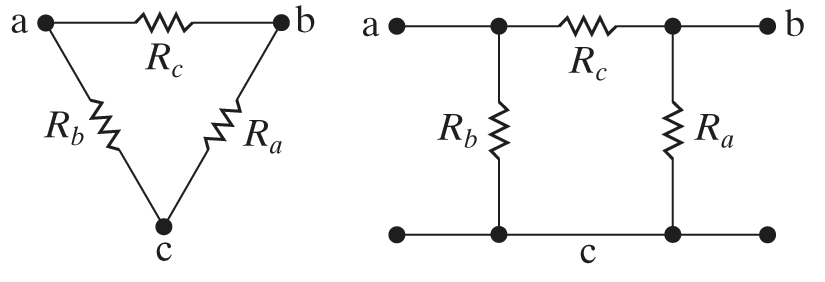
\includegraphics[scale=0.50]{fig/fig03_32.png}
\caption{$\Delta$ configuration viewed as a $\pi$ configuration}
\label{fig:fig03_32}
\end{center}
\end{figure}

Another configuration is the wye ($Y$) or the electrically equivalent tee ($T$) interconnection

\begin{figure}[H]
\begin{center}
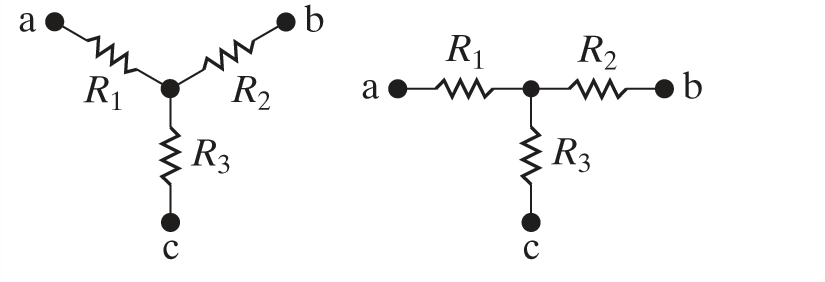
\includegraphics[scale=0.50]{fig/fig03_33.png}
\caption{$Y$ configuration viewed as a $T$ configuration}
\label{fig:fig03_33}
\end{center}
\end{figure}

\subsection{The Delta to Y transformation}

\begin{figure}[H]
\begin{center}
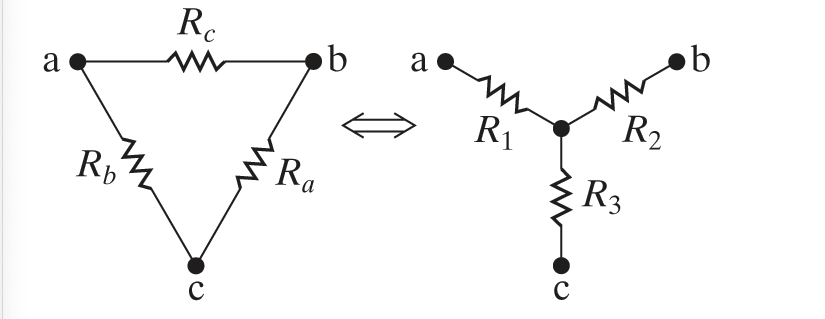
\includegraphics[scale=0.50]{fig/fig03_34.png}
\caption{$\Delta$ to $Y$ Transformation}
\label{fig:fig03_34}
\end{center}
\end{figure}

The resistance between terminals needs to be the same whether they are in series or parallel. The three equivalent resistance equations are:

\begin{equation}
R_{ab} = \frac{R_c (R_a + R_b)}{R_a +R_b + R_c} = R_1 + R_2
\end{equation}

\begin{equation}
R_{bc} = \frac{R_a (R_b + R_c)}{R_a +R_b + R_c} = R_2 + R_3
\end{equation}

\begin{equation}
R_{ca} = \frac{R_b (R_c + R_a)}{R_a +R_b + R_c} = R_3 + R_1
\end{equation}

Through algebraic manipulation

\begin{equation}
R_1 = \frac{R_b R_c}{R_a + R_b + R_c}
\end{equation}

\begin{equation}
R_2 = \frac{R_c R_a}{R_a + R_b + R_c}
\end{equation}

\begin{equation}
R_3 = \frac{R_a R_b}{R_a + R_b + R_c}
\end{equation}

Or this can be reversed

\begin{equation}
R_a = \frac{R_1 R_2 + R_2 R_3 + R_3 R_1}{R_1}
\end{equation}

\begin{equation}
R_b = \frac{R_1 R_2 + R_2 R_3 + R_3 R_1}{R_2}
\end{equation}

\begin{equation}
R_c = \frac{R_1 R_2 + R_2 R_3 + R_3 R_1}{R_3}
\end{equation}


\begin{tcolorbox}
Do Example 3.11
\end{tcolorbox}


\chapter{Techniques of Circuit Analysis}

\section{Terminology}

\begin{figure}[H]
\begin{center}
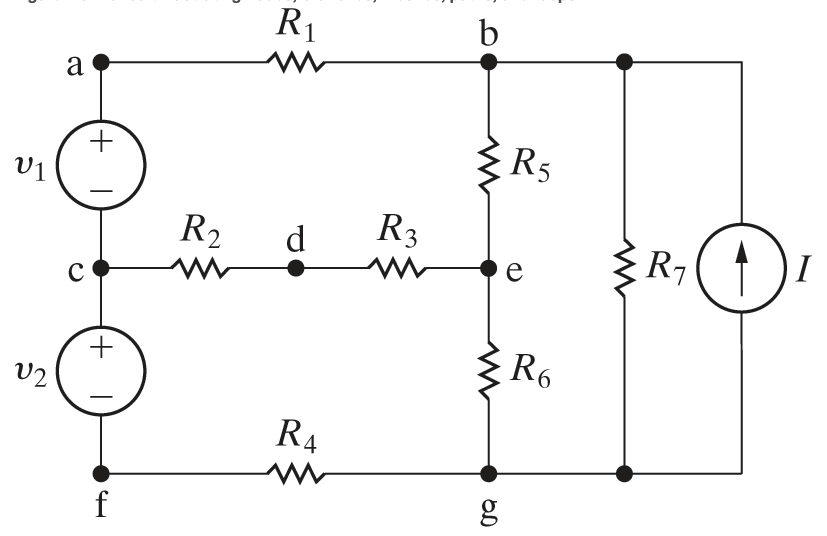
\includegraphics[scale=0.50]{fig/fig04_03.png}
\caption{Terminology Diagram}
\label{fig:fig04_03}
\end{center}
\end{figure}

\begin{table}[]
\begin{tabular}{|l|l|l|}
\hline
Name                                                        & Definition                                                                                                                      & Example                   \\ \hline
node                                                        & A point where two or more elements join                                                                                         & a                         \\ \hline
\begin{tabular}[c]{@{}l@{}}essential \\ node\end{tabular}   & A node where three or more elements join                                                                                        & b                         \\ \hline
path                                                        & \begin{tabular}[c]{@{}l@{}}A trace of adjoining basic circuit elements \\ with no elements included more than once\end{tabular} & $v_1 - R_1 - R_2 -R_3$    \\ \hline
branch                                                      & A path that connects two nodes                                                                                                  & $R_1$                     \\ \hline
\begin{tabular}[c]{@{}l@{}}essential \\ branch\end{tabular} & \begin{tabular}[c]{@{}l@{}}A path that connects two essential nodes\\ without passing through an essential node\end{tabular}    & $v_1 - R_1$               \\ \hline
loop                                                        & \begin{tabular}[c]{@{}l@{}}A path whose last node is the same as \\ the starting node\end{tabular}                              & $v_1-R_1-R_5-R_6-R_4-v_2$ \\ \hline
mesh                                                        & A loop that does not enclose any other loops                                                                                    & $v_1-R_1-R_3-R_2$         \\ \hline
\begin{tabular}[c]{@{}l@{}}planar \\ circuit\end{tabular}   & \begin{tabular}[c]{@{}l@{}}A circuit that can be drawn on a plane \\ with no crossing branches\end{tabular}                     & see figures               \\ \hline
\end{tabular}
\end{table}

\begin{figure}[H]
\begin{center}
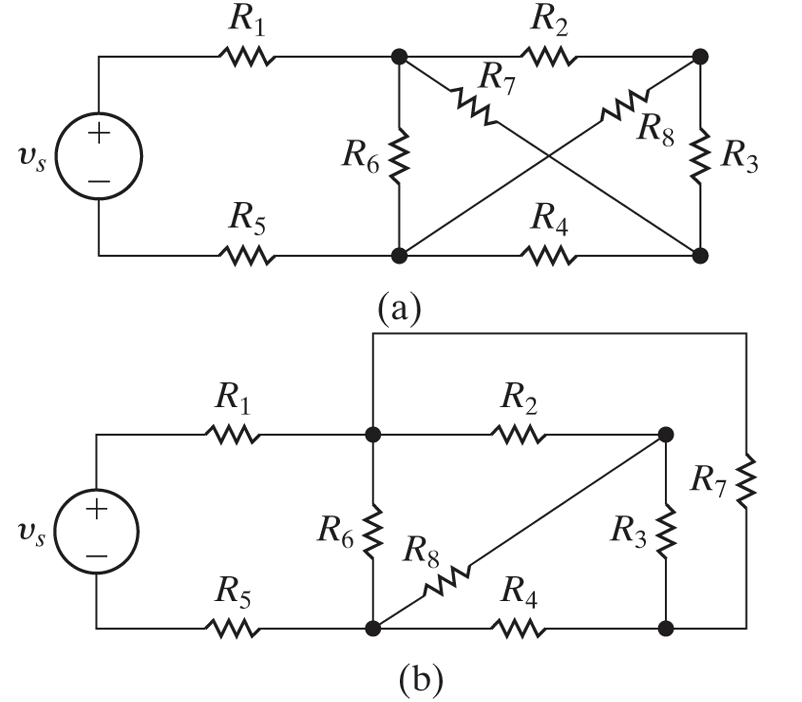
\includegraphics[scale=0.50]{fig/fig04_01.png}
\caption{Planar Circuit}
\label{fig:fig04_01}
\end{center}
\end{figure}

\begin{figure}[H]
\begin{center}
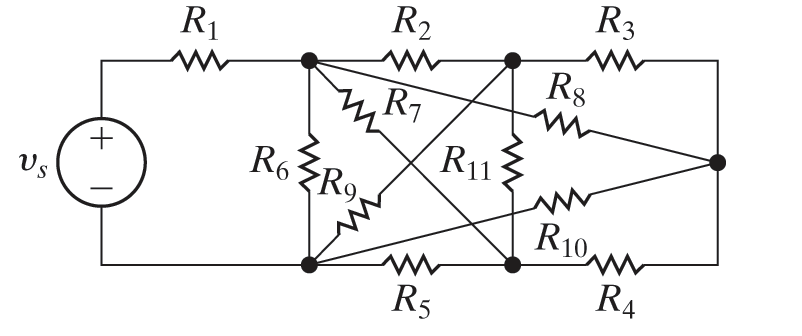
\includegraphics[scale=0.50]{fig/fig04_02.png}
\caption{Non Planar Circuit}
\label{fig:fig04_02}
\end{center}
\end{figure}

\begin{tcolorbox}
Do Example 4.1
\end{tcolorbox}


\subsection{Simultaneous Equations}

Recall that you need $x$ independent equations to solve a circuit with $x$ unknown currents.

Method:
\begin{itemize}
\item Count the number of essential nodes, $n_e$
\item Count the number of essential branches, $b_e$, where the current is \underline{unknown}.
\item Write $n_e - 1$ equations by applying KCL to any set of $n_e - 1$ nodes.
\item Write $b_e - (n_e - 1)$ equations by applying KVL around a set of $b_e - (n_e - 1)$ loops or meshes. 
\end{itemize}

Note - the voltage for each element in every loop or mesh must be known or must be described in terms of current using Ohm's law.

\begin{tcolorbox}
Do Example 4.2
\end{tcolorbox}

\section{Node-Voltage Method}

\begin{enumerate}
\item Identify the essential nodes
\item Pick and label a reference node, then label the node voltages at the remaining essential nodes. 
\item Write a KCL equation for every non-reference essential node
\item Solve the equations to find the node-voltage values
\item Sove the circuit using the node voltages from Step 4 to find the component currents, voltages, and power values.  
\end{enumerate}

\begin{tcolorbox}
Do Example 4.3
\end{tcolorbox}


\begin{tcolorbox}
Do Assessment Problem 4.1


Left Node:
\begin{equation}
15 = i_{60} + i_{15} + i_1
\end{equation}

\begin{equation}
15 = \frac{v_1}{60} + \frac{v_1}{15} + \frac{v_1 - v_2}{5}
\end{equation}

\begin{equation}
\frac{17}{60} v_1 - \frac{12}{60} v_2 = 15
\end{equation}

Right Node:
\begin{equation}
i_1 = i_2 + 5
\end{equation}

\begin{equation}
 \frac{v_1 - v_2}{5} = \frac{v_2}{2} + 5
\end{equation}

\begin{equation}
\frac{1}{5} v_1 - \frac{7}{10} v_2 = 5
\end{equation}

Combining:

\begin{equation}
A = 
\begin{bmatrix}
0.2833 & -0.2000 & | & 15 \\
0.2000 & -0.7000 & | &  5 
\end{bmatrix}
\end{equation}

Using in Octave rref(A):

\begin{equation}
rref(A) = 
\begin{bmatrix}
1 & 0 & | & 60 \\
0 & 1 & | & 10 
\end{bmatrix}
\end{equation}

\begin{equation}
v_1 = 60 V, 
v_2 = 10 V, 
i_i = 5 A
\end{equation}



\end{tcolorbox}

\section{Node-Voltage Method and Dependent Sources}

If the circuit contains dependent sources, the KCL equations must be supplemented with the constraint equations imposed by the dependent sources. The Step 3 of the Node-Voltage method is modified as seen in the example below.

\begin{tcolorbox}
Do Example 4.4
\end{tcolorbox}

\begin{tcolorbox}
Do Assessment Problem 4.3
\end{tcolorbox}

\section{Node-Voltage Method - Special Cases}

\subsection{Known Voltages}
\begin{tcolorbox}
Do Example with Figure 4.12
\end{tcolorbox}

\subsection{Supernodes}
When a voltage source is between two essentail nodes, we can combine those nodes and the source to form a supernode.

\begin{tcolorbox}
Do Example with Figure 4.15
\end{tcolorbox}

\begin{tcolorbox}
Do Example 4.5 - Node-Voltage Analysis of an Amplifier Circuit
\end{tcolorbox}

\section{Mesh-Current Method}
\begin{tcolorbox}
\begin{center}
Caution: this only works for Planar Circuits
\end{center}
\end{tcolorbox}


The Mesh-Current Method
\begin{enumerate}
\item Identify the meshes with curved directed arrows that follow the perimeter of each mesh
\item Label th emesh currents for each mesh
\item Write a KVL equation for each mesh
\item Solve the equations to find the mesh current values
\item Sove the circuit using the mesh currents from Step 4 to find the component currents, voltages, and power values.  
\end{enumerate}

\begin{tcolorbox}
Do Example 4.6
\end{tcolorbox}

\begin{tcolorbox}
Do Assessment Problem 4.7
\end{tcolorbox}

\section{The Mesh-Current Method and Dependent Sources}

\begin{tcolorbox}
Do Example 4.7
\end{tcolorbox}


\section{The Mesh-Current Method: Special Cases}

\subsection{Known Current}
\begin{tcolorbox}
Do Example 4.8
\end{tcolorbox}

\subsection{Supermesh}
When a current source is shared between two meshes, we can combine the meshes to form a supermesh.

\begin{tcolorbox}
Do Example with Figure 4.28
\end{tcolorbox}

\section{Source Transformations}

\begin{figure}[H]
\begin{center}
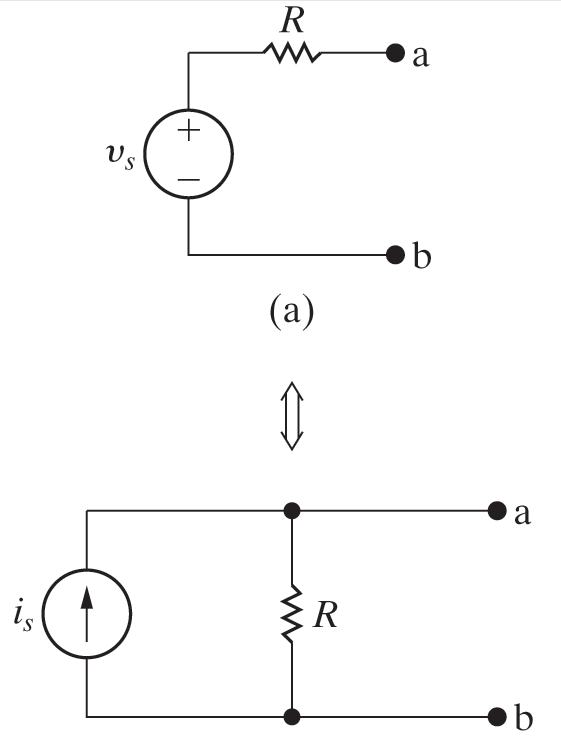
\includegraphics[scale=0.50]{fig/fig04_38.png}
\caption{Source Transformations}
\label{fig:fig04_38}
\end{center}
\end{figure}


Supposed we connect Resistor $R_L$ between Nodes A and B:

From the voltage source figure,
\begin{equation}
i_L = \frac{v_s}{R + R_L}
\end{equation}

And, from the current source figure,
\begin{equation}
i_L = \frac{R}{R + R_L} i_s
\end{equation}

Which leads to
\begin{equation}
i_s = \frac{v_s}{R}
\end{equation}

\begin{tcolorbox}
Do Example 4.12
\end{tcolorbox}

\section{Thevenin and Norton Equivalent Circuits}

\subsection{Thevenin Equivalent Circuit}

Any circuit that contains linear elements can be represented by a Thevenin Equivalent Circuit that is the series combination of a voltage source $V_{TH}$ and a resistor $R_{TH}$.

\begin{figure}[H]
\begin{center}
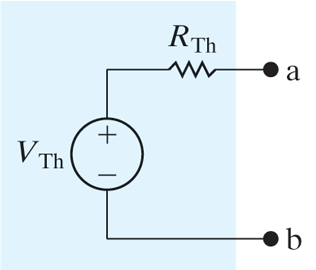
\includegraphics[scale=0.50]{fig/fig04_46.png}
\caption{Thevenin Equivalent Circuit}
\label{fig:fig04_46}
\end{center}
\end{figure}

To calculate $V_{Th}$ we assume the load resistance is infinitely large (i.e., an open circuit) and calculate $V_{Th}$:

\begin{equation}
V_{Th} = V_{oc}
\end{equation} 

Next, we reduce the load resistance to zero (i.e., short circuit) and find $i_{sc}$.

Given that 
\begin{equation}
i_{sc} = \frac{V_{Th}}{R_{Th}}
\end{equation}
We find that
\begin{equation}
R_{TH} = \frac{V_{Th}}{i_{sc}}
\end{equation}

\begin{tcolorbox}
Do Example 4.14
\end{tcolorbox}


\subsection{Norton Equivalent Circuit}

Similarly, we can create a Norton Equivalent Circuit

\begin{figure}[H]
\begin{center}
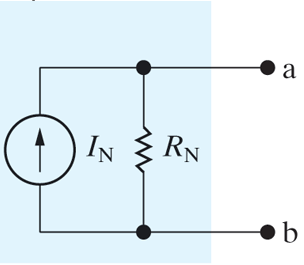
\includegraphics[scale=0.50]{fig/fig04_50.png}
\caption{Norton Equivalent Circuit}
\label{fig:fig04_50}
\end{center}
\end{figure}

\begin{equation}
I_N = i_{sc}
\end{equation}

and

\begin{equation}
R_N = \frac{v_{oc}}{i_{sc}} = R_{Th}
\end{equation}

\begin{tcolorbox}
Do Example 4.15
\end{tcolorbox}

\section{Maximum Power Transfer}

\begin{figure}[H]
\begin{center}
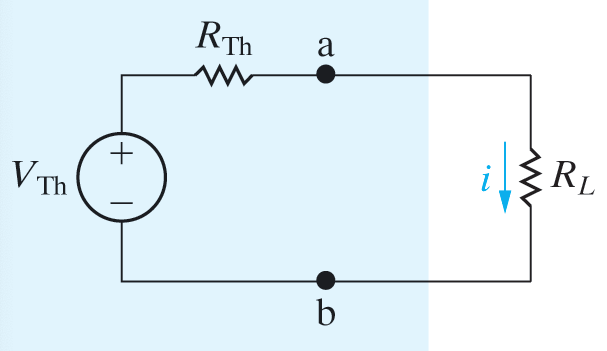
\includegraphics[scale=0.50]{fig/fig04_64.png}
\caption{Max Power Transfer}
\label{fig:fig04_64}
\end{center}
\end{figure}

\begin{equation}
p = i^2 R_L = (\frac{V_{Th}}{R_{Th} + R_L})^2 R_L
\end{equation}

Take the derivative

\begin{equation}
\frac{dp}{dR_L} = V^2_{Th} [\frac{(R_{Th} + R_L)^2 - 2 R_L (R_{Th} + R_L)}{(R_{Th} + R_L)^4}
\end{equation}

Find where the derivative is zero:
\begin{equation}
(R_{Th} + R_L)^2 = 2 R_L (R_{Th} + R_L)
\end{equation}

Solving for $R_L$ yields
\begin{equation}
R_L = R_{Th}
\end{equation}

And the maximum power transferred to a resistive load

\begin{equation}
p_{max} = \frac{V^2_{Th}}{4 R_L}
\end{equation}

\begin{tcolorbox}
Do Example 4.21
\end{tcolorbox}

\section{Superposition}
A linear system obeys the principle of superposition, which states that whenever a linear system is excited, or driven, b more than one independent source of energy, the total response is the sum of the individual responses. 


\begin{tcolorbox}
Do Example 4.22
\end{tcolorbox}
\appendix

\chapter{Integration by Trig Substitution}
\label{sec:trigsub}

Find the integral of 

\begin{equation}
\int \frac{1}{(a^2 + x^2)^{\frac{3}{2}}}
\end{equation}

Integrate by trig substitution by setting $x = a\tan{u}$ which leads to 

\begin{equation}
\frac{dx}{du} = \frac{a \tan{u}}{du} = \frac{a}{\cos^2{u}}
\end{equation}

Which leads to 
\begin{equation}
dx = ( \frac{a}{\cos^2{u}}) du 
\end{equation}

Thus

\begin{equation}
\int \frac{1}{(a^2 + x^2)^{\frac{3}{2}}} =  \int \frac{1}{(a^2 + (a\tan{(u)})^2)^{\frac{3}{2}}} ( \frac{a}{\cos^2{(u)}}) du
\end{equation}

\begin{equation}
=  \int \frac{1}{(a^2)^{\frac{3}{2}} (1 + \tan^2{(u)})^{\frac{3}{2}}} ( \frac{a}{\cos^2{(u)}}) du
\end{equation}

\begin{equation}
=  \int \frac{1}{(a^3)(\frac{1}{\cos^2(u)})^{\frac{3}{2}}} ( \frac{a}{\cos^2{(u)}}) du
\end{equation}

\begin{equation}
=  \frac{1}{a^2} \int \frac{1}{(\frac{1}{\cos^2(u)})^{\frac{3}{2}}} ( \frac{1}{\cos^2{(u)}}) du
\end{equation}

\begin{equation}
=  \frac{1}{a^2} \int \frac{1}{(\frac{1}{\cos^3(u)})} ( \frac{1}{\cos^2{(u)}}) du
\end{equation}

\begin{equation}
=  \frac{1}{a^2} \int \cos{(u)} du
\end{equation}

\begin{equation}
=  \frac{1}{a^2} \sin{(u)} + C
\end{equation}


From the above $\arctan{(\frac{x}{a})} = u$ so

\begin{equation}
=  \frac{1}{a^2} \sin{(\arctan{(\frac{x}{a})})} + C
\end{equation}

\begin{equation}
=  \frac{1}{a^2} [\frac{\frac{x}{a}}{\sqrt{1+(\frac{x}{a})^2}}] + C
\end{equation}

\begin{equation}
=  \frac{x}{a^3} [\frac{1}{\frac{1}{a} \sqrt{a^2+x^2}}] + C
\end{equation}

Which finally leads to

\begin{equation}
\int \frac{1}{(a^2 + x^2)^{\frac{3}{2}}} =  \frac{x}{a^2} [\frac{1}{\sqrt{a^2+x^2}}] + C
\end{equation}





\chapter{Chain Rule}

\begin{equation}
\frac{d}{dx} (\frac{1}{\sqrt{x^2+R^2}}) = \frac{d}{dx} (x^2+R^2)^{-\frac{1}{2}} 
\end{equation}

The chain rule $ f(g(x))' = f'(g(x) \cdot g'(x)$. In this case $g(x) = x^2 + R^2$. From this

\begin{equation}
f(g(x)) = g(x)^{-\frac{1}{2}} 
\end{equation}

thus  

\begin{equation}
f'(g(x)) = -\frac{1}{2} g(x)^{-\frac{3}{2}} 
\end{equation}

and

\begin{equation}
g'(x) = 2x
\end{equation}

Thus

\begin{equation}
f(g(x))' =  -\frac{1}{2} g(x)^{-\frac{3}{2}}  \cdot 2x
\end{equation}

\begin{equation}
\frac{d}{dx} (\frac{1}{\sqrt{x^2+R^2}}) = \frac{-x}{(x^2 + R^2)^\frac{3}{2}}
\end{equation}


\end{document}
